\section{Instrumentation}
\label{instrumentation}

In order to detect muon and electron events, signals from scintillators are correlated and matched against an expected pattern. The next section (\ref{procedure}) will discuss how these are used to generate lifetimes; here, we focus on describing the apparatus and problems associated with it.

\subsection{Scintillators}
\label{scintillators}

The scintillator consists of polystyrene ($\mathrm{C}_{8}\mathrm{H}_{9}$, with density $1.08 \pm .09 \frac{\mathrm{g}}{\mathrm{cm}^{3}}$) doped with a phosphorous material, p-terphenyl. When ionizing radiation passes through the material a light pulse is emitted. The light flash is detected by the photomultiplier tubes placed at the ends of the scintillator. The photomultiplier uses a high voltage (on the order of 1000 V) to convert the light pulses into a cascade of electrons more or less linearly (i.e., the amplitude of the electrical signal from the photomultiplier is linearly correlated to the energy of the ionizing radiation). The signals from the photomultiplier is then fed into a bank of discriminators, which output a fixed width voltage pulse after detecting a voltage pulse above a given threshold. These signals are then fed into the logic which determines events. For the muon mass measurement, the discriminated signals are still used to mark events, but the raw output of the photomultiplier is viewed directly so as to determine the energy of the passing muon.

\subsubsection{Photomultiplier False Flashes}
\label{photomultiplierfalseflashes}

Photomultipliers, while incredibly useful and sensitive in delivering amplified event signals, have a notorious weakness: false signals which occur with some regularity directly after real signals. The number of these signals, as detailed in the autocorrelator section of Appendix~\ref{muontimeerroranalysis}, follows a more or less exponential decay (that is, there are exponentially fewer false pulses at longer times than shorter times); however, the decay lifetime is of approximately the same order of magnitude as the lifetime of the muons. Different techniques, described below (\ref{efficiencyoptimization}) and in the \emph{Procedure} section (\ref{muonlifetimemeasurement}), were used to lower the effect of these false signals; however, they remain a significant pollutant of data in the low end of the timescale, and must be dealt with statistically (see Appendix~\ref{muontimeerroranalysis}).

\subsubsection{Efficiency Optimization}
\label{efficiencyoptimization}

Many different factors come into the consideration for choosing the settings at which the run the scintillators. The most obvious is the desire to maximize efficiency of the detectors so as to maximize muon count; this would require setting the voltages as high as possible and the threshold levels as low as possible. The other primary concern is noise (particularly false flashes), which increases at higher voltages and lower thresholds; this concern keeps voltages lower and thresholds higher. An optimization procedure determines the optimal settings to maximize efficiency.

The optimization technique relies on the very high number of muons that go straight through all detectors. As most muons are very high energy when they reach the surface of the earth, nearly the entire flux from the atmosphere passes through all the detectors without stopping. Thus, by taking the ratio of the number of events detected by all three detectors as compared to the number detected by just two of the detectors, we can get an approximation of the efficiency of the excluded detector, as any event detected by just the two should have been detected by all three. The ratio should be near 1 for something perfectly efficient, as losses from solid angles and muons which stop in the detectors are incredibly small as compared to the total muon flux. We chose the most efficient detector to be in the middle, as most of the signals require at least one middle input.

Optimal voltage values are chosen by plotting efficiency against voltage; this produces a plot that increases dramatically at low voltages but soon plateaus. A value in the middle of this plateau is chosen to guarantee the high rate of efficiency, but not so high as to increase noise. Optimal values for discriminator threshold levels were chosen in a similar fashion; a plot of threshold versus efficiency showed a plateau as discriminator levels are lowered. Once again a middle value on the plateau is chosen, in an attempt to balance guaranteeing high efficiency with noise concerns.

Initial data runs were taken with very high efficiency: $99\%$ efficiency for the middle detector, $83\%$ for the top, and $90\%$ for the bottom. Voltages for the photomultiplier tubes were set at 1160 V, 1190 V, and 1190 V respectively. All the thresholds were set to 70 mV. 

After the discovery of noise problems detailed above and in Appendix~\ref{muontimeerroranalysis}, the efficiency of the detectors was lowered considerably, to $91\%$, $70\%$, and $78\%$. Voltages were changed to 1140 V, 1160 V, and 1130 V, with thresholds raised uniformly to 100 mV.

\subsection{Logic}
\label{logic}

In order to register muon events, signals are fed out of the discriminator into a series of logic banks. For example, to register a muon passing all the way through (used in optimizations and muon mass measurements), the equation $T \wedge M \wedge B$ is used: that is, all three signals are anded together. Any time that all three detectors flash simultaneously, it is clear that a muon has passed through all of them. It is unlikely that two separate muon events will be anded; about 50 muons pass through the scintillators in one second, so we expect real muon events every .02 s. Pulses out of the discriminator, on the other hand, are set to 100 ns for the top and bottom and 50 ns for the middle (set differently in order to guarantee overlap); thus, since pulses are several orders of magnitude quicker than the rate of incoming muons, we expect very few overlap errors. Furthermore, time of flight values for muons and electrons traveling between the scintillators are negligible; see Appendix~\ref{timeofflight}.

The muon lifetime measurement requires a signal that indicates a muon has stopped in the middle scintillator; we call this event START, as this would start the lifetime count. The signal is simply given by $\mathrm{START} = T \wedge M \wedge \bar{B}$; that is, a signal is detected on the top and middle detectors but not the bottom. This either means that the muon has stopped in the middle detector, or gone past the bottom detector at an angle; because of the close distances between the scintillators (on the order of cm), this later case is unlikely, and we can interpret the event as a stopped muon.

Similarly, the muon lifetime measurement also requires a stop signal. The stop would occur after the decay has happened; that is, an electron has been detected. After the muon decays, the electron can move off in any direction (since the muon was at rest, and the neutrinos take care of momentum conservation), but generally speaking we can expect the electron to be detected not just at the middle detector, but the top or bottom one as well (since most electrons will have some vertical component in their momentum, and given the size of the scintillators, a small amount of vertical momentum will result in the electron striking the detector). Thus, a simple STOP event would be defined as: $\mathrm{STOP} = (T \wedge M \wedge \bar{B}) \vee (\bar{T} \wedge M \wedge B)$; that is, a stop event is either a bottom going or top going event.

However, this allows for START and STOP events to happen simultaneously: note that STOP is actually defined by a START event or'ed with a different event. Moreover, consider the scenario in which a muon stops in the middle detector, but the resulting electron actually comes out the side; instead of admitting that there was no STOP detected, the next START event would be recorded as a STOP. Thus, we should redefine STOP to occur only after a valid START, within some acceptable timeframe. The logic diagram in Figure~\ref{figure:logic} illustrates the solution: STOP as it is currently defined is anded with a delayed gate signal (that is, a delayed signal set constantly high, set to expire after a given amount of time) that is triggered by a START event. The delay to the start of the gate is set to 100 ns, twice as long as the 50 ns pulses outputted by the logic units, guaranteeing that simultaneous events will not trigger a measurement; the gate length is set to $20 \mu s$, 10 times the expected lifetime: waiting any longer is likely waiting for an electron which went out in an undetected fashion.

\begin{figure}[htbp]
\begin{center}
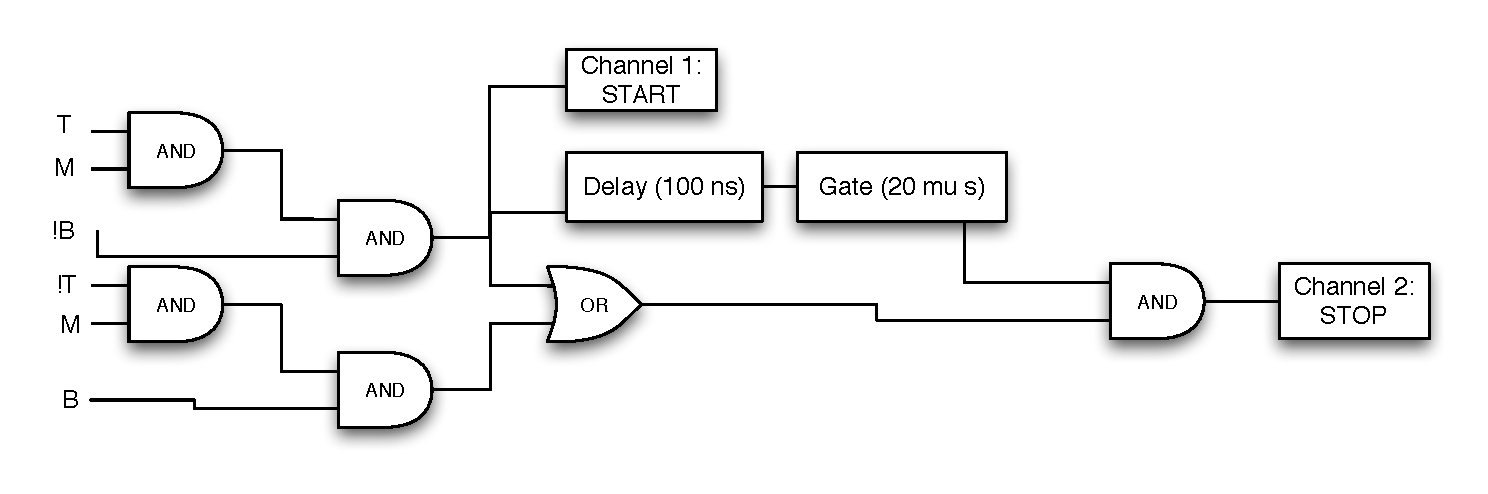
\includegraphics[height=50mm]{./figures/logicdiagram.eps}
\caption{Complete logic diagram for muon lifetime measurement}
\label{figure:logic}
\end{center}
\end{figure}


\subsection{Autocorrelator}
\label{autocorrelator}
In order to better study the effects of the photomultiplier false flashes, we used a Langley Ford Instruments Model 1096 Correlator to track the autocorrelation of the signal coming from each photomultiplier. The machine monitors at an input line for a signal, and records when another signal comes onto the same channel. We set it to record bins of $.1 \mu$s, up to a total of $8 \mu$s after the starting signal. Because the rate of muons coming into a scintillator is significantly smaller than this timescale, any autocorrelated signals could be strongly assumed to be false flashes (indeed, if there were extra muons coming in during this window, we would expect an even distribution over all times, but we did not see this). The results were normalized by dividing by the total number of signals detected over the run period.

\subsection{Measurements}
\label{measurements}
To make measurements, a LabView program takes data from an oscilloscope over a GPIB connection. For the lifetime experiment, the oscilloscope is set to trigger on a stop event, and the program measures the difference in time between the beginnings of the start and stop pulses, on channel 1 and 2 of the oscilloscope respectively. For the mass experiment, the scope is set to monitor for a trigger on channel 2 (a logic pulse indicating the required condition) and to monitor the height of pulses on channel 1 (the actual output from the photomultiplier).